\begin{figure*}
\centering
\includegraphics[width=0.7\textwidth]{figures/process.pdf}
\label{fig:process}
\caption{Three-step process for generating a control plane that generates
    policy-compliant paths under bounded failures}
\end{figure*}

\section{Control Plane Synthesis via ARCs} \label{sec:synthesis}
In this section, we describe preliminary ideas on how each phase of our synthesis 
approach is implemented.
First, we briefly discuss how existing tools can be used to generate
policy-compliant paths (\secref{TODO}).
Second, we show how to generate ARCs that induce
the set of paths synthesized in the first phase (\secref{TODO}).
Third, we show how ARCs can be modified to deal with resilience (\secref{TODO}).
Finally, we show how to restart the process whenever one of the three phases fails (\secref{TODO}).

\subsection{From policies to paths}
Synthesizing sets of paths---i.e., data planes---that adhere to a given set of policies
is already a hard problem, but a few practical approaches have been proposed.
The approach that better meets our policy language is the one proposed in Merlin~\cite{}.
Merlin supports waypoints, reachability policies, and restricted forms of traffic engineering. 
Merlin uses automata to succinctly represent
the set of all possible paths reachability and waypoint policies and then mixed integer linear programming
to identify a concrete set of paths meeting the traffic engineering requirements.
We implemented a similar approach in our prototype tool. 
Since this part of the problem is not novel, we briefly provide the intuition behind our solution.
Our approach directly uses  constraint solving to generate paths adhering to the given policies and does 
not use automata operations to describe the search space. This choice is dictated by the complex set of policies, such as isolation,
that our tool wants to support. 
Given a set of policies we 
use an encoding similar to that of Merlin to generate a set of constraints over the propositional theory of
rationals. Every solution to this set of constraints is a set of paths satisfying the given policies.

\loris{we will add more details if needed}


\subsection{From paths to ARCs}

We first describe the synthesis of a type of ARC 
called {\em pure} ARC which
only forwards packet bases on shortest-paths and does 
not support additional mechanisms like filtering etc. 
Thus, 
the ARC is a directed graph comprising switches as 
vertices and weighted edges corresponding to all links in the
topology (no link is disabled by any mechanism). 
This is 
a ideal control plane because it is able to enforce the data plane
with carefully engineered edge weights and no links are disabled. 
For a given network data plane, the synthesis of 
the pure ARC from input paths reduces to a
variation of the {\em inverse shortest path} problem, an almost 
unexplored algorithmic problem. 

Formally, this variation of inverse shortest path problem 
has as input: (1) a directed graph $T = (S, L)$ (the network topology), 
(2) a set of endpoints $\Gamma \subseteq S\times S$, and 
(3) a set of paths $P \subset L*$
such that for each $(s,t) \in \Gamma, \exists p \in P$ such
that the path $p$ is a set of links connecting $s$ to $t$. 
The problem is to find weights for the edges $L$ such that 
for each $(s,t) \in \Gamma$, every lowest weighted path 
in the graph 
from $s$ to $t$ is in the set $P$. 

Since, the forwarding is destination-based,
for a destination $d$, we aggregate the paths 
to create a directed graph $\xi_d$ with the destination
as the sink. Since, the forwarding path cannot have 
loops, $\xi_d$ must be a directed acyclic graph for 
correct enforcement, else we reject the input if this
requirement is not adhered to.
We define $\Omega$ for the 
set of destinations, and $\Delta$ for  
the set of destination DAGs. 
Given $\Omega$ and $\Delta$, we generate a set of linear equations
to find the requisite edge weights of a pure ARC. 
For this, we define $E(sw_1, sw_2)$ as
the edge weight variable for link $sw_1 \rightarrow sw_2$. 
We use $\rightarrow$ operator to denote a path of length 1 
(link), $\rightarrow^*$ to denote a path of length $\geq 0$
and $\rightarrow^+$ to denote a path of length $\geq 1$.
For a path connecting two switches 
$s \rightarrow^+ t$ in a DAG, 
to enforce that the path will be the shortest, we need equations
which ensure the sum of edge weights of the path is strictly smaller than
the weight of all other paths from $s$ to $t$. 

\minisection{Distance Equations}
$D(s,t)$ denotes the absolute shortest distance from $s$ to $t$. 
Trivially, $D(s,s) = 0$. For a path $s \rightarrow^+ t$ ($len \geq 1$),
the shortest distance from $s$ to $t$ is the smallest of the distances
of the paths traversed through the neighbours of $s$ to $t$. The
following equations enforce the semantics of distances; 
here $s \rightarrow sw$ denotes that $sw$ is a neighbour
of $s$, and $sw \rightarrow^* t$ denotes that the path from $sw$ to $t$ contains
zero or more edges.
\begin{multline} \label{eq:dist}
\forall s, t, sw. (s \rightarrow sw \rightarrow^* t).\\
D(s, t) \leq E(s, sw) + D(sw, t)
\end{multline}
Intuitively, $D(s,t)$ is not greater than 
the actual shortest distance from $s$ to $t$.

\minisection{Destination DAG Equations}
For each destination DAG, we add equations to ensure the 
edge weights are set such that a shortest-path forwarding in the ARC 
follows the same path or paths specified in the DAG. If a path
is the shortest path between its endpoints, then every 
subpath of the path has to be the shortest between its endpoints
as well (otherwise the complete path would not be the shortest).
\begin{figure}[h!] 
	\centering
	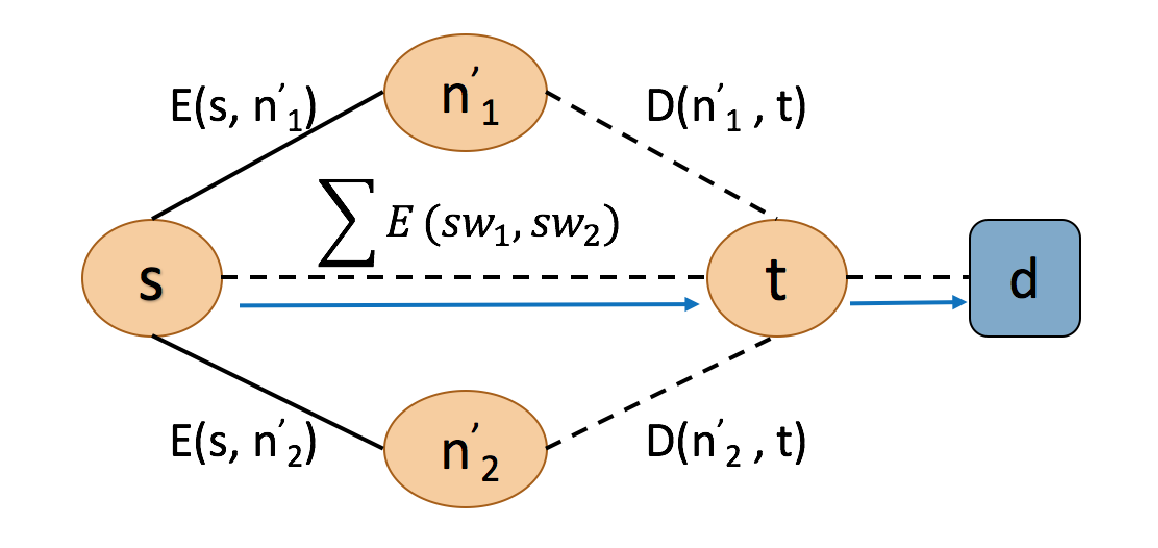
\includegraphics[width=0.8\columnwidth]{figures/distanceEquation.eps}
	\caption{Distance equation} \label{fig:disteq}
\end{figure}
Consider a DAG $\xi_d$ for destination $d$. We define two neighbour
functions: $N(s)$ denotes the set of neighbours of switch $s$ 
in the directed graph, and $N(s, \xi_d)$ denote the set of
neighbours of switch $s$ in the destination DAG. 
Consider a path $s \rightarrow^+ t$ in the DAG ($t$ 
need not be the destination. As the DAG specifies
the shortest paths to the destination, this 
path from $s$ to $t$ has the lowest weight, 
which we express by the sum of weights of 
edges along the path. 
To satisfy the semantics of the ARC,
we need to ensure that all other
paths from $s$ to $t$ are have strictly 
greater path weights.
Thus, we add the following equations to ensure the
shortest path property (\Cref{fig:disteq} illustrates 
an example).
\begin{multline} \label{eq:uniq}
		\forall d \in \Omega. \forall s, t \in \xi_d. (s \rightarrow^+ t).\\ 
		\forall n'. (n' \in N(s) \wedge n' \not\in N(s, \xi_d)). \\
		\sum_{\mathclap{\substack{(sw_1, sw_2) \in (s \rightarrow^+ t)}}} 
		E(sw_1, sw_2) < E(s, n') + D(n', t)
\end{multline}
By using distance for the path $n' \rightarrow t$, we 
are able to find lower bounds to the weight of the non-DAG 
paths from $s$ to $t$,
thus avoiding the blow-up of enumerating all paths from $s$
to $t$. 

% If the path $n' \rightarrow^* t$ 
% is not in any DAG completely, then
% $D(n',t)$ can be smaller than the actual shortest distance by the
% semantics of \Cref{eq:dist} (as
% $D(n',t)$ is not equal to any quantity by \Cref{eq:shortest}).
% However, since $D(n',t)$ is on the RHS of the equations in \Cref{eq:uniq},
% the equations will ensure that the path $s\rightarrow n \rightarrow^* t$
% has strictly greater weight than the path of the DAG.

%TODO: Add some figures
